\begin{figure*}
\begin{center}
\centerline{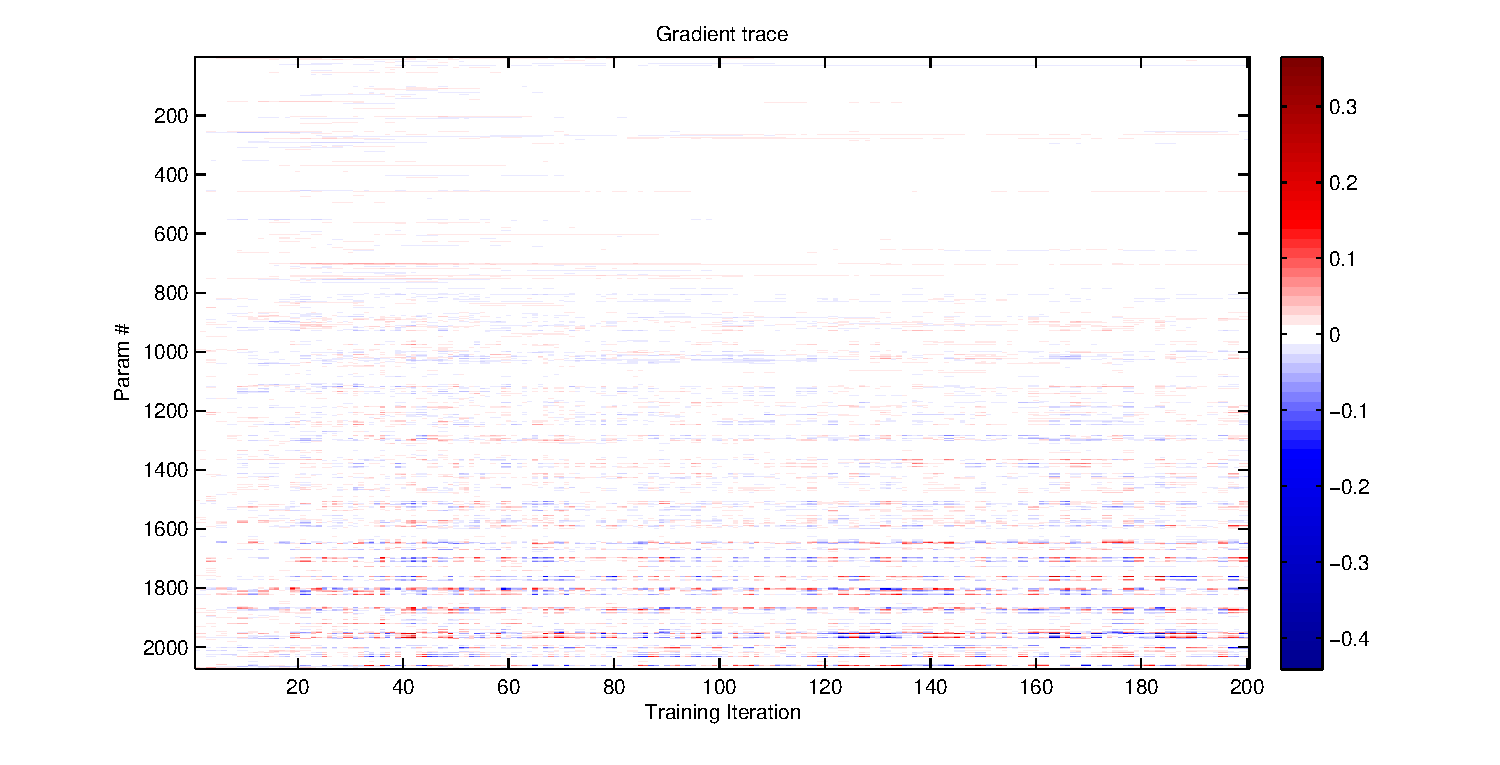
\includegraphics[width=\linewidth]{ppt1}}
\caption{Gradident trace sampled every 100 iterations during optimization of a
network with 5 hidden layers each with 16 units. White is small or zero
gradient, thus alternating red and blue implies oscillation. The gradient
vector at each time step is plotted such that lower down corresponds to weights
at a higher layer in the network.}
\label{gradt}
\end{center}
\end{figure*}

\begin{figure*}
\begin{center}
\centerline{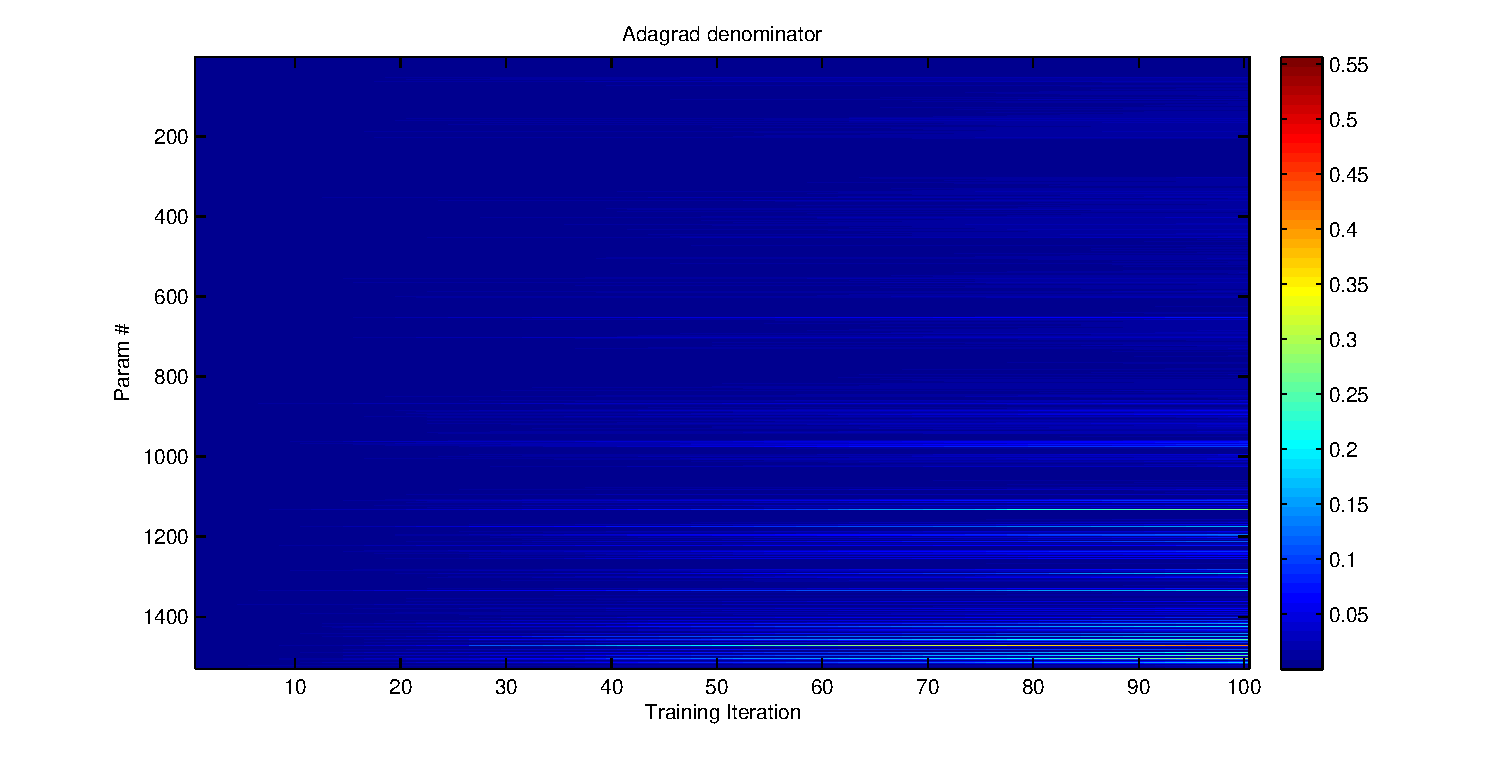
\includegraphics[width=\linewidth]{ppt2}}
\caption{Trace of the diagonal of the matrix $G_t$ used in the AdaGrad update.
Network details are the same as in \ref{gradt}. We note clear nondecreasing
monotonicity of the components of this vector.}
\label{adagradt}
\end{center}
\end{figure*}

\begin{figure*}[ht!]
\begin{center}
\centerline{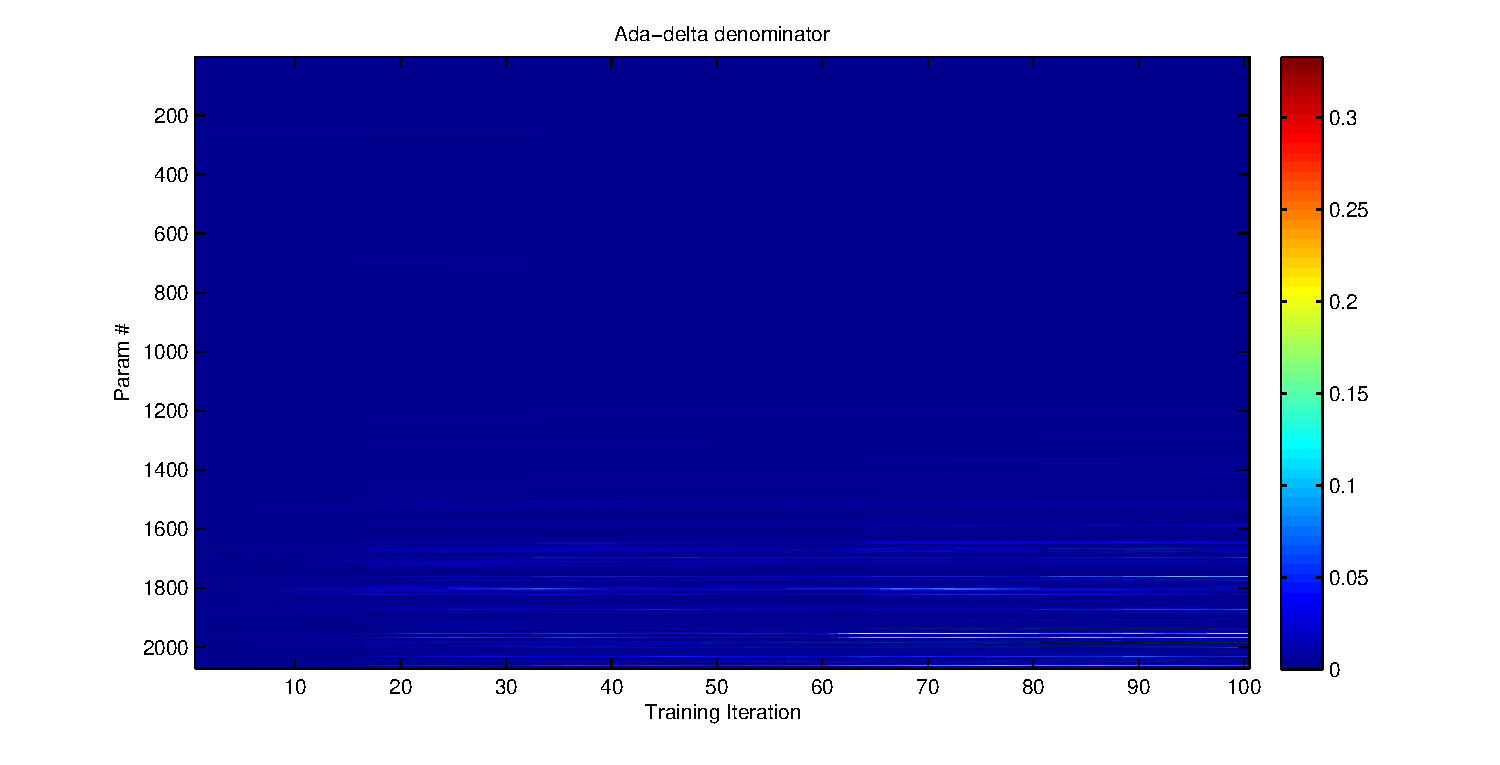
\includegraphics[width=\linewidth]{ppt3}}
\caption{Trace of the diagonal of the matrix $G_t$ used in the AdaGrad update
with decay parameter $\gamma=0.99$. Network details are the same as in
\ref{gradt}.}
\label{adadeltt}
\end{center}
\end{figure*}

\begin{figure*}[ht]
\begin{center}
\centerline{\includegraphics[scale=1]{mnist_ae_adagrad_lrs}}
\caption{Learning curves for the AdaGrad optimizer with different global step size $\eta$. The autoencoder is the same as in Figure \ref{mnist_ae}.}
\label{mnist_ae_adagrad_lrs}
\end{center}
\end{figure*}

\begin{figure*}[ht]
\begin{center}
\centerline{\includegraphics[scale=1]{mnist_ae_nesterov_lrs}}
\caption{Learning curves for the Nesterov optimizer with different global step sizes $\eta$ and a fixed momentum of $\mu=0.99$. The autoencoder is the same as in Figure \ref{mnist_ae}.}
\label{mnist_ae_nesterov_lrs}
\end{center}
\end{figure*}

\begin{figure*}[ht]
\begin{center}
\centerline{\includegraphics[scale=1]{mnist_ae_adadelta_lrs}}
\caption{Learning curves for the decayed version of AdaGrad, $\gamma=0.99$, with different global step sizes $\eta$. The autoencoder is the same as in Figure \ref{mnist_ae}.}
\label{mnist_ae_adadelta_lrs}
\end{center}
\end{figure*}

